\documentclass{article}

\usepackage[T1]{fontenc}
\usepackage[utf8]{inputenc}
\usepackage{lmodern}
\usepackage{amsmath}
\usepackage{graphicx}
\usepackage{bm}
\usepackage{fancyvrb}

\author{Sigrid Videm}
\title{Project 2}

\begin{document}
\maketitle
\tableofcontents % for a table of contents

\section{Abstract} 
The aim of this project is to solve the Schroedinger equation for a particle in a potential well. The equation is scaled and rewritten as an eigenvalue problem, and I have used the Jacobi method to find eigenvalues and eigenvectors. The eigenvalues will give the energies of the eigen states, the eigenvector will give the radial probability. Later, I used the same algorithm for solving the two particle problem. The only change I needed to do was to use a different discretization matrix. 
\section{Introduction}
In this project I have a made program that uses Jacobi's method for finding eigenvalues. The method is described in the Methods section. This program can be used for finding eigenvalues of all symmetric matrices, but here I have focused on finding the eigenvalues of a matrix which is a discretization of the Schrodinger equation for one and two electrons in a potential well.  I have used a scaled version of the equation. This makes the program suitable for solving other problems involving the wave equation with fixed boundaries. The scaling and discretization is briefly explained in the Methods section. In the Results section, there are plots of the eigenvectors for the three lowest eigenvalues for the one particle case. This is interpreted as the radial probability distribution. There is also a short discussion of efficiency and the choise of boundary values and number of mesh points. In the two particle case I focus on the relative coordinate of the two particles, and investigate hwo the probability distribution depends on the potential strength $\omega_r$. Plots of the three solutions with the lowest eigenvalues are in the Results section.

My code is available at https://github.com/sigrivi/Project2

\section{Method}
\subsection{Scaling and discretization of the Scrodinger equation}

I am going to solve the radial part Schroedinger's equation for one electron: 
$$
  -\frac{\hbar^2}{2 m} \left ( \frac{1}{r^2} \frac{d}{dr} r^2
  \frac{d}{dr} - \frac{l (l + 1)}{r^2} \right )R(r) 
     + V(r) R(r) = E R(r).
$$
In the project description(\cite{Projectdescription}) it is shown that when $l=0$ we can scale the equation and discretize it. With scaling constants
\begin{equation*}
\alpha = \left(\frac{\hbar^2}{mk}\right)^{1/4}.
\end{equation*}
and

\begin{equation*}
\lambda = \frac{2m\alpha^2}{\hbar^2}E,
\end{equation*}
we can rewrite Schroedinger's equation as

\begin{equation*}
  -\frac{d^2}{d\rho^2} u(\rho) + \rho^2u(\rho)  = \lambda u(\rho) .
\end{equation*}
Discretizing the equation gives the matrix eigenvalue problem:
$$
\begin{bmatrix} \frac{2}{h^2}+V_1 & -\frac{1}{h^2} & 0   & 0    & \dots  &0     & 0 \\
                                -\frac{1}{h^2} & \frac{2}{h^2}+V_2 & -\frac{1}{h^2} & 0    & \dots  &0     &0 \\
                                0   & -\frac{1}{h^2} & \frac{2}{h^2}+V_3 & -\frac{1}{h^2}  &0       &\dots & 0\\
                                \dots  & \dots & \dots & \dots  &\dots      &\dots & \dots\\
                                0   & \dots & \dots & \dots  &-\frac{1}{h^2}  &\frac{2}{h^2}+V_{N-2} & -\frac{1}{h^2}\\
                                0   & \dots & \dots & \dots  &\dots       &-\frac{1}{h^2} & \frac{2}{h^2}+V_{N-1}
             \end{bmatrix}  \begin{bmatrix} u_{0} \\
                                                              u_{1} \\
                                                              \dots\\ \dots\\ \dots\\
                                                              u_{N}
             \end{bmatrix}=\lambda \begin{bmatrix} u_{0} \\
                                                              u_{1} \\
                                                              \dots\\ \dots\\ \dots\\
                                                              u_{N}
             \end{bmatrix}.  
$$

The eigenvalue problem has $n$ eigenvalues $\lambda_i$ and $n$ eigenvectors  $({\bm{x}_1},\ldots,\bm{x}_n)$. The energy of each state is 
$$E_n=\frac{{\hbar}^2}{2m{\alpha}^2}{\lambda}_n$$
and the probability distribution is ${x_i}^2$. To solve this problem, I will use Jacobi's rotational algorithm.  

\subsection{Jacobi's method}
The idea behind Jacobi's method is that an orthogonal transformation does not change the dot product. To show this:
Let the vectors $\bm{v_i}$ be the vectors of an orthogonal basis. Then $\bm{v_j}^T\bm{v_i}=\delta_{ij}$. Let $\bm{U}$ be an orthogonal matrix, that is $\bm{U}^T\bm{U}=\bm{I}$. The orthogonal transformation $\bm{w_i}=\bm{Uv_i}$ preserves the dot product:  
$$\bm{w_j}^T\bm{w_i}= \bm{v_j}^T\bm{U}^T\bm{Uv_i}=\bm{v_j}^T\bm{Iv_i}=\bm{v_j}^T\bm{v_i}=\delta_{ij}$$ Since the dot product is preserved, the vectors $\bm{w_j}$ also form an orthogonal basis.

This means that if we start out with the eigenvalue problem $\bm{Ax}=\lambda\bm{x}$, a series of unitary transformations on $\bm{A}$ will not change the eigenvalues $\lambda$ (but they change the eigenvectors $\bm{x}$). The orthogonal transformations of the Jacobi method rotates the matrix around an angle $\theta$. This is done by multiplying the equation with a rotation matrix $\bm{S}$. $\bm{S}$ is the identity matrix, except for 
$$s_{kk}=s_{ll} =\cos \theta$$
$$s_{lk} = -s_{lk} =\sin \theta $$

When the matrix $\bm{A}$ is rotated arond an angle $\theta$, the elements of the new matrix $\bm{B}$ are given by:
$$
b_{ii} = a_{ii} 
$$$$
b_{ik} = a_{ik} \cos{\theta}-a_{il}\sin{\theta} 
$$$$
b_{kk} = a_{kk} \cos^2{\theta}-2a_{kl} \cos{\theta} \sin{\theta}+a_{ll} \sin^2{\theta}
$$$$
b_{ll} = a_{ll}  \cos^2{\theta}+2a_{kl} \cos{\theta} \sin{\theta}+a_{kk} \sin^2{\theta}
$$$$
b_{lk} = (a_{kk}-a_{ll})\cos{\theta} \sin{\theta}+a_{kl}(\cos^2{\theta}-\sin^2{\theta})
$$
We want to choose $\theta$ so that $b_{kl}=0$:
$$
0=(a_{kk}-a_{ll})\cos{\theta} \sin{\theta}+a_{kl}(\cos^2{\theta}-\sin^2{\theta})
$$$$
0=\frac{a_{kk}-a_{ll}}{2a_{kl}}\tan{\theta}+\frac{1}{2}-\frac{1}{2}\tan^2{\theta}
$$
With $t=\tan{\theta}$ and $\tau=\frac{a_{kk}-a_{ll}}{2a_{kl}}$, $\tan{\theta}$ is the solution of the equation $$0=\frac{1}{2}t^2-\tau t-\frac{1}{2}$$  This equation has two solutions, $t=\tau\pm \sqrt{{\tau}^2+1}$. At every iteration I used the smallest value of $t$  to calculate the elements of $\bm{B}$:
$$
b_{ii} = a_{ii} 
$$$$
b_{ik} = (a_{ik}-a_{il}t )(t^2+1)^{-\frac{1}{2}}
$$$$
b_{kk} = (a_{kk}-2a_{kl} t+a_{ll} t^2)(t^2+1)^{-1}
$$$$
b_{ll} = (a_{ll} +2a_{kl} t+a_{kk} t^2)(t^2+1)^{-1}
$$
Because the matrix is symmetric, $b_{lk}=b_{kl}=0$ , $b_{ki}=b_{ik}$ and $b_{li}=b_{il}$.

The eigenvectors are also transformed. I stored the eigenvectors $\bm{x_i}$ as columns in a matrix $\bm{X}$, and I used $\bm{X}=\bm{I}$ as an initial value. The multiplication with the rotation matrix $\bm{S}$ results in a new matrix $\bm{Y}$, with elements:
$$
y_{ik}=\cos{\theta}x_{ik}-\sin{\theta}x_{il}
$$

$$
y_{il}=\cos{\theta}x_{il}+\sin{\theta}i_{ik}
$$

The code I used for the rotation:
\begin{verbatim}
def rotate_A(A, X, k, l): #rotates matrix A around an angle theta. 
	
	N = A.shape[0]
	B = A.copy()
	tau = ( A[k,k]-A[l,l] )/( 2*A[k,l] )
	if A[k,k]-A[l,l] == 0:
		print(" A[k,k]-A[l,l] = 0")
	if A[k,l] ==0:
		print("A[kl}=0")

	t1 = tau - math.sqrt( tau**2+1 ) # t=tan(theta)
	t2 = tau + math.sqrt( tau**2+1 )
	t = t1
	
	if t2**2 < t1**2: #choose the smaller value of t1 and t2
		t = t2
	
	c = (t**2+1)**(-0.5) ## c = cos(theta)
	s = c*t ## s = sin(theta)
	
	Y = X.copy() #matrix of eigen vectors

	for i in range(N):
		if (i!=l and i!=k):
			B[i,k] = (A[i,k]-A[i,l]*t)*(t**2+1)**(-0.5)
			B[i,l] = (A[i,l]+A[i,k]*t)*(t**2+1)**(-0.5)
			B[k,i] = B[i,k]
			B[l,i] = B[i,l]

		Y[i,k] = c*X[i,k] - s*X[i,l] 
		Y[i,l] = c*X[i,l] + s*X[i,k]

	B[l,l] = (A[l,l] + 2*A[k,l]*t + A[k,k]*t**2)/(t**2+1)
	B[k,k] = (A[k,k] - 2*A[k,l]*t + A[l,l]*t**2)/(t**2+1)
	B[k,l] = 0
	B[l,k] = 0

	return(B,Y)

\end{verbatim}
The function rotate\_A is called many times, untill all non-digaonal elements were smaller than a value $\epsilon=10^{-8}$. The eigenvalues are the diagonal elements of of the matrix $ \bm{B} $, and the eigenvectors are the columns of the matrix $ \bm{Y} $. To get the three smallest eigenvalues and their eigenvectors, I made a function to sort the eigenvalues. 
\begin{verbatim}
def eigenvalues_and_eigenvectors(A, epsilon):
	
	B, X, iterations = jacobi(A,epsilon) #B is the matrix with eigenvalues along diagonal, X is the matrix of eigenvectors
	print("iteration:", iterations)
	eigenvalues = B.diagonal() #eigenvalues is a vector of eigenvalues
	eig_sort = np.sort( eigenvalues )
	index = np.argsort (eigenvalues )
	X=X.transpose() #the eigenvectors are now rows in X
	eigenvector = np.zeros((B.shape[0],B.shape[1]))
	for i in range(B.shape[0]):
		eigenvector[i,:] = X[index[i],:]
	
	return(eig_sort, eigenvector)
\end{verbatim}

To get the eigenvalues and eigenvectors of the groud state: 
\begin{verbatim}
eig_val, eig_vec = eigenvalues_and_eigenvectors(A, 1.e-8)
eig_val[0] 
eig_vec[0]
\end{verbatim}
The rest of the code is found in project2b\_ alt.py. (project2b.py is a program which only finds eigenvalues, and not eigenvectors). Unit tests are found in project2\_ unittests.py.

In the results section, plots of the wave functions for the three lowest eigenvalues are presented, followd by a discussion of how the eigenvectors depends on $\rho_N$ and number of mesh points needed and run time of the program. 

\subsection{Scaling an discretization in the two particle case}
I used the same program for the two particle case, but with a different matrix $\bm{A}$. In the project description (\cite{Projectdescription}) 	I found the scaling constants 

\begin{equation*}
\omega_r^2=\frac{1}{4}\frac{mk}{\hbar^2} \alpha^4,
\end{equation*}

\begin{equation*}
\alpha = \frac{\hbar^2}{m\beta e^2}.
\end{equation*}


\begin{equation*}
\lambda = \frac{m\alpha^2}{\hbar^2}E,
\end{equation*}


Here, the diagonal elements of $\bm{A}$ have $V_i = \omega_r ^2 {\rho_i}^2+\frac{1}{\rho_i}$. $\omega_r$ reflects the strength of the potential well, and I found the eigenvalues and eigenvectors for different $\omega_r$. Plots of probability distributions are found in the results section. The code used for this part is in project\_ 2d.py



\section{Results and discussion}
\subsection{The one particle case}
Figure \ref{fig:one_electron} shows the radial probability distribution for the three lowest energy states of a particle in a potential well. The corresponding theoretical eigenvalues are $\lambda_0=3$, $\lambda_1=7$ and $\lambda_2 =11$. The energies of these states can be calculated by 
$$E_n=\frac{{\hbar}^2}{2m{\alpha}^2}{\lambda}_n$$ 
Figure \ref{fig:one_electron} shows that for the lowest energy, we can expect to find the particle on a sphere of radius $r=\alpha \rho$. For energy state $n$, there are $n+1$ radii where we can expect to find the particle.
In my calculations of eigenvalues and eigenvectors I chose $\rho_N=5$. With this value of $\rho_N$, all three functions approaches zero when $\rho\rightarrow \rho_N$. With a smaller $\rho_N$, I will lose the tail, and a larger $\rho_N$ will make the tail unneccessarily long.  
I ran the program with different numbers of mesh points, and compared the run time with that of the Python eigenvalue solver. As shown in table \ref{tab:table1}, the Jacobi algorithm is much slower. Based on the data in the table, I find that the number of iterations grows as $N^2 \cdot \frac{5}{3}$.
 With 200 mesh points, I found the three lowest eigenvalues to be $\lambda_0=2.9998$, $\lambda_1=6.9990$ and $\lambda_2 =10.9978$. This is an accuracy of approximately four leading digits after the decimal point. I used $N=200$ for the plot in figure \ref{fig:one_electron}.

\begin{table}[h!]
  \centering
  \caption{Run time and number of iterations for solving the eigenvalue problem depending on the number of mesh points $N$}
  \label{tab:table1}
  \begin{tabular}{l||l|l|l}
   $N$ & run time Jacobi & number of iterations Jacobi & run time Python solver\\

    \hline
    50  & 1.038 s & 4046 & 0.0008 s \\
    \hline
    100 & 8.4608 s & 16531 & 0.0023 s \\
    \hline
     150 & 28.8550 s & 37350 & 0.0041 s \\
	\hline
	200 & 70.4640 s & 66617 & 0.0126 s \\
  \end{tabular}
\end{table}



\begin{figure}
  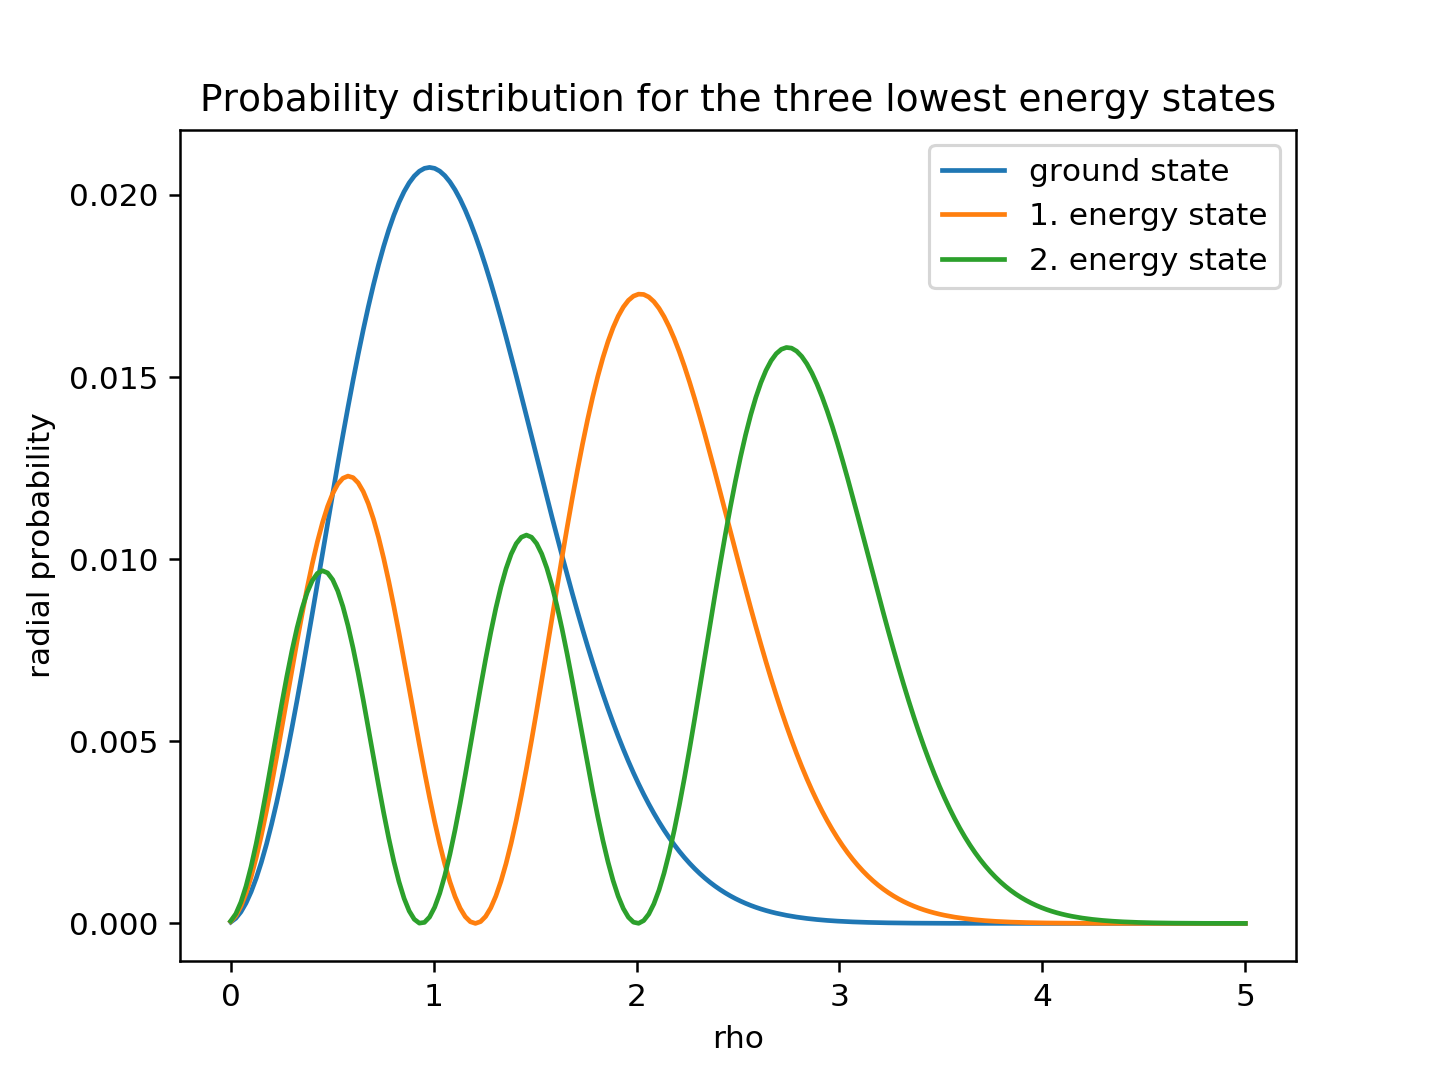
\includegraphics[width=\linewidth]{one_electron.png}
  \caption{The probability distribution for the three lowest energy states of one electron in a potential well.}
  \label{fig:one_electron}
\end{figure}

\subsection{The two particle case}
In the two particle case, I used $\rho_N=5,10,15$, and I used $N=100$ to make the computations faster. Table \ref{tab:table2} shows that the eigenvalues $\lambda_0$, $\lambda_1$ and $\lambda_2$ when $\omega_r =0.25$. The eigenvalues are appriximately equal for $\rho_N=10$ and $\rho_N=15$, but differs when $\rho_N=5$. For this reason, I used $\rho_N=15$ for the plots in figure \ref{fig:ground_state}, \ref{fig:first_state}, \ref{fig:second_state}. The figures shows that when the potential strength $\omega_r$ is large, the relative coordinate is small, and the electrons will be close to each other in spite of the electric repulsion. 

\begin{table}[h!]
  \centering
  \caption{Eigenvalues calculated with different $\rho_N$ and $\omega_r =0.25$.}
  \label{tab:table2}
  \begin{tabular}{l||l|l|l}
   $\rho_N$ & $\lambda_0$ & $\lambda_1$ & $\lambda_2$\\

    \hline
    15  & 1.24922611183 & 2.18656472194 & 3.14171419782 \\
    \hline
    10 & 1.24980673783 & 2.18923192551 & 3.14842559179 \\
    \hline
     5 & 1.30427183063 & 2.65683356456 & 4.681720701 \\

  \end{tabular}
\end{table}
For $\omega_r=0.25$ and $\omega_r=0.05$ M. Taut (\cite{Oscillatorfrequancies}) have found theoretical values for the eigenvalue of the ground state. Table \ref{tab:table3} shows these values, along with the values I have found, using $N=100$. 

\begin{table}[h!]
  \centering
  \caption{Eigenvalues calculated with different $\rho_N$ and $\omega_r =0.25$.}
  \label{tab:table3}
  \begin{tabular}{l||l|l|l}
  $\omega_r$ & theoretical $\lambda_0$ & numerical $\lambda_0$ & relative error\\

    \hline
    0.25  & 1.25 & 1.249226 & 0.00062 \\
    \hline
    0.05 & 0.35 & 0.350832 & 0.0023 \\
    

  \end{tabular}
\end{table}



    
Because the relative error is small for $\omega_r=0.25$, I used this value for comparing the eigenvalues for different $\rho_N$ (which was done in table \ref{tab:table2}). The relative error is larger when $\omega_r$ is smaller. To get  better value for $\lambda_0$, I think I have to increase $\rho_N$, because a weak potential will give a longer relative distance. 

\begin{figure}
  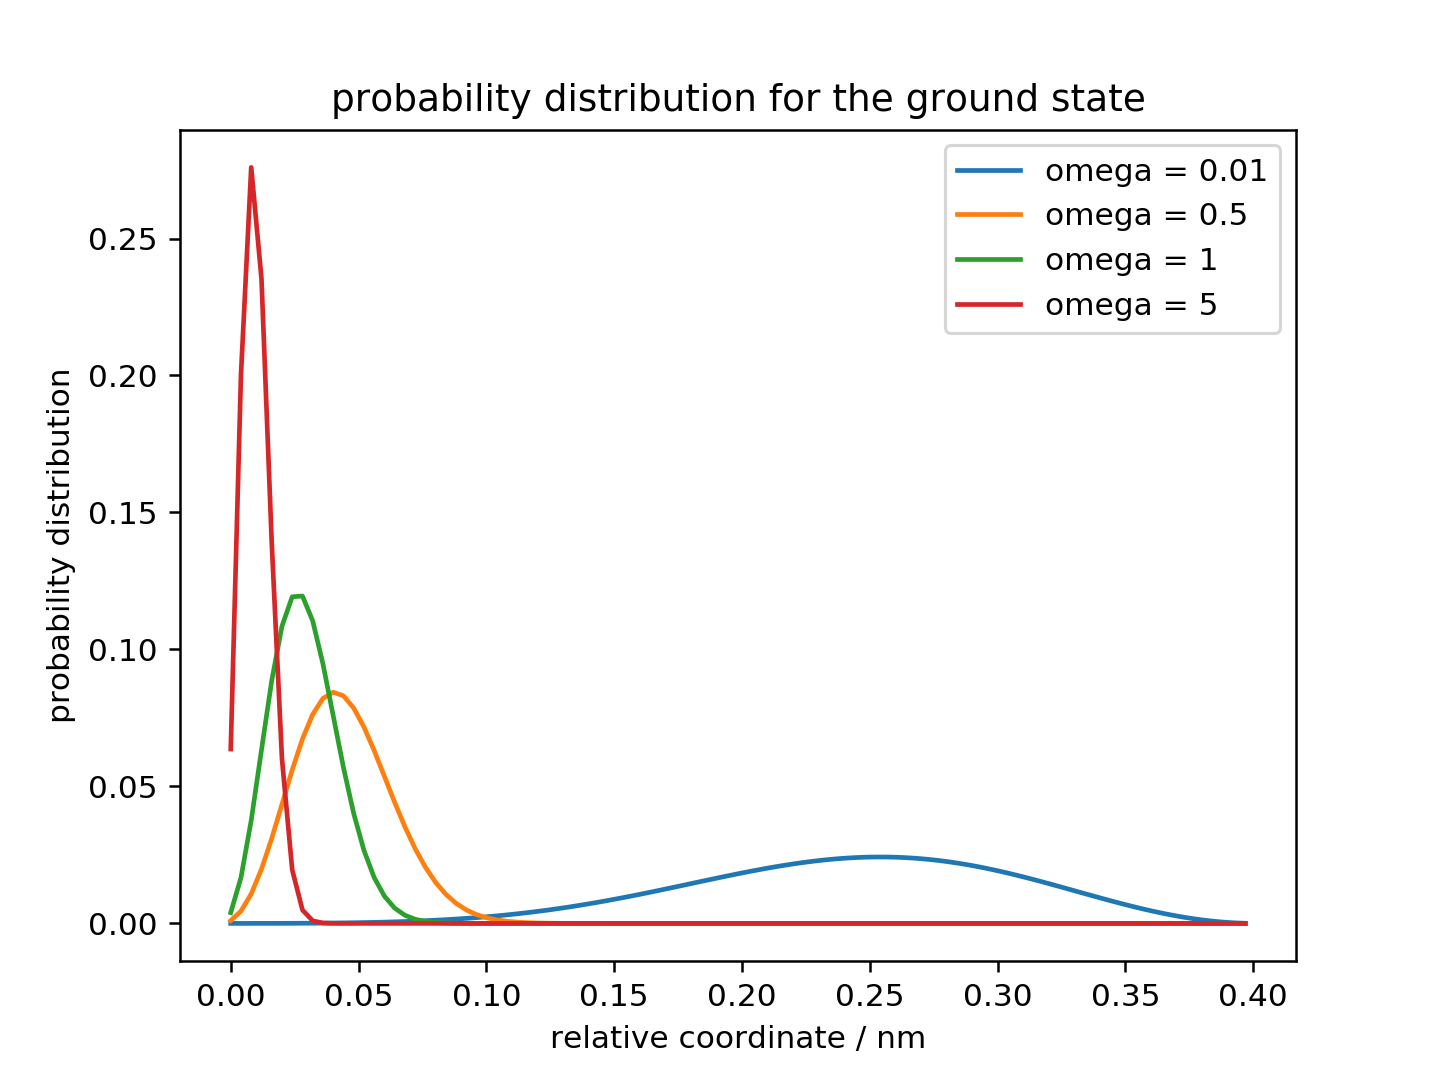
\includegraphics[width=\linewidth]{ground_state.png}
  \caption{The probability distribution for two electrons in a potential well, for different potential stengths}
  \label{fig:ground_state}
\end{figure}

\begin{figure}
  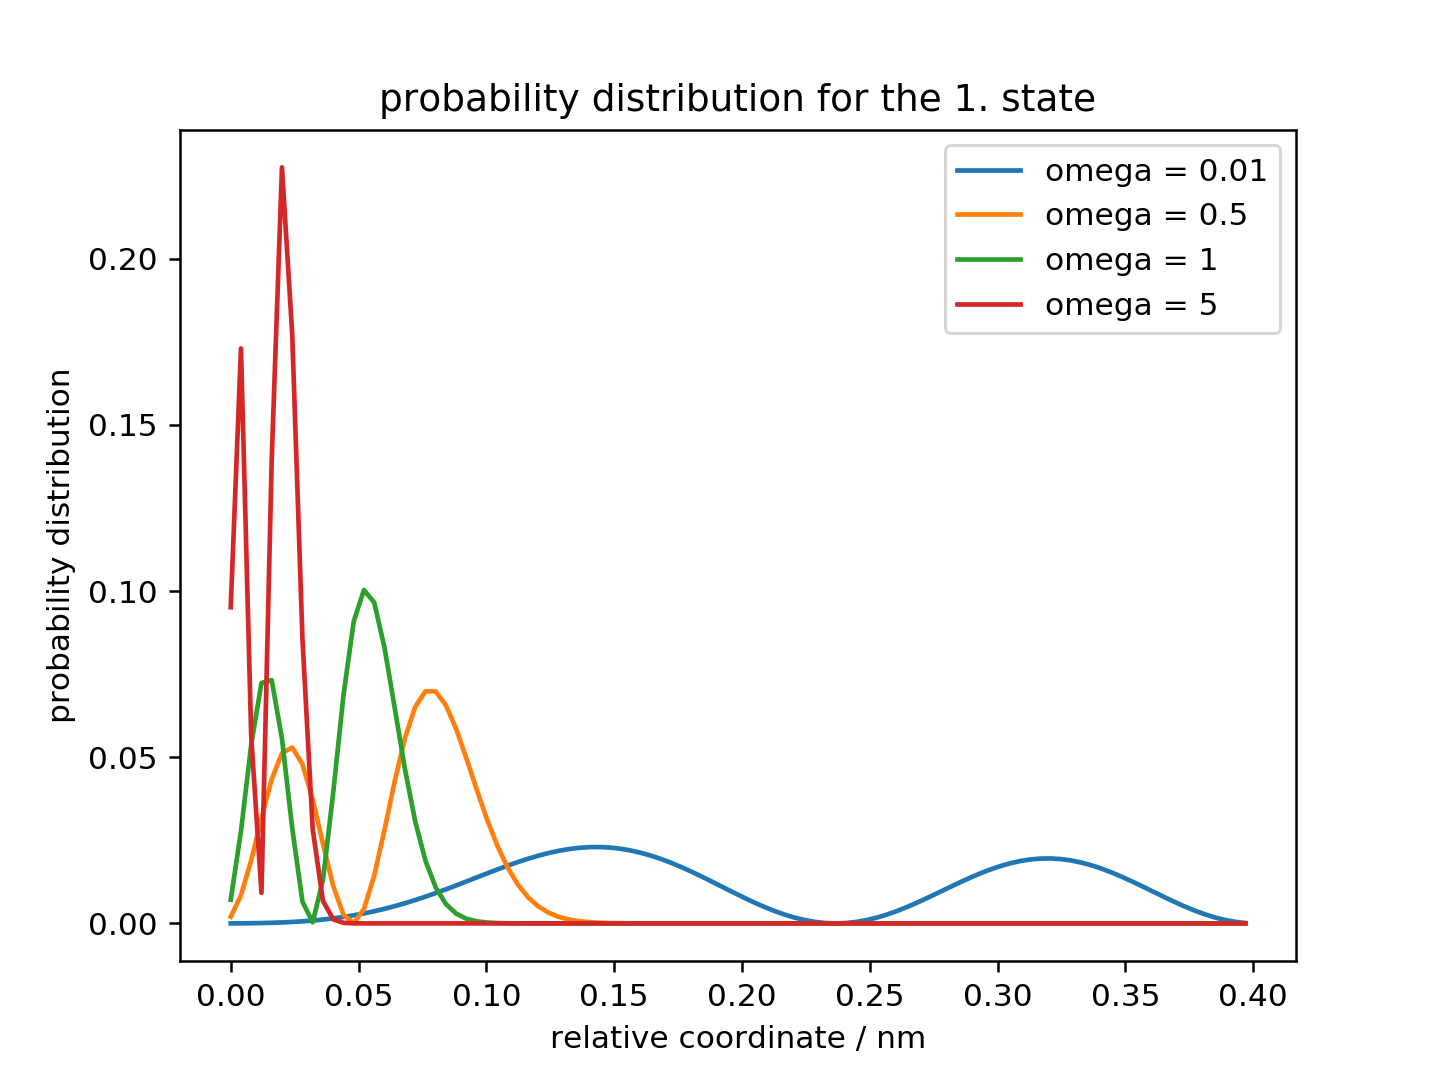
\includegraphics[width=\linewidth]{first_state.png}
  \caption{The probability distribution for two electrons in a potential well, for different potential stengths}
  \label{fig:first_state}
\end{figure}

\begin{figure}
  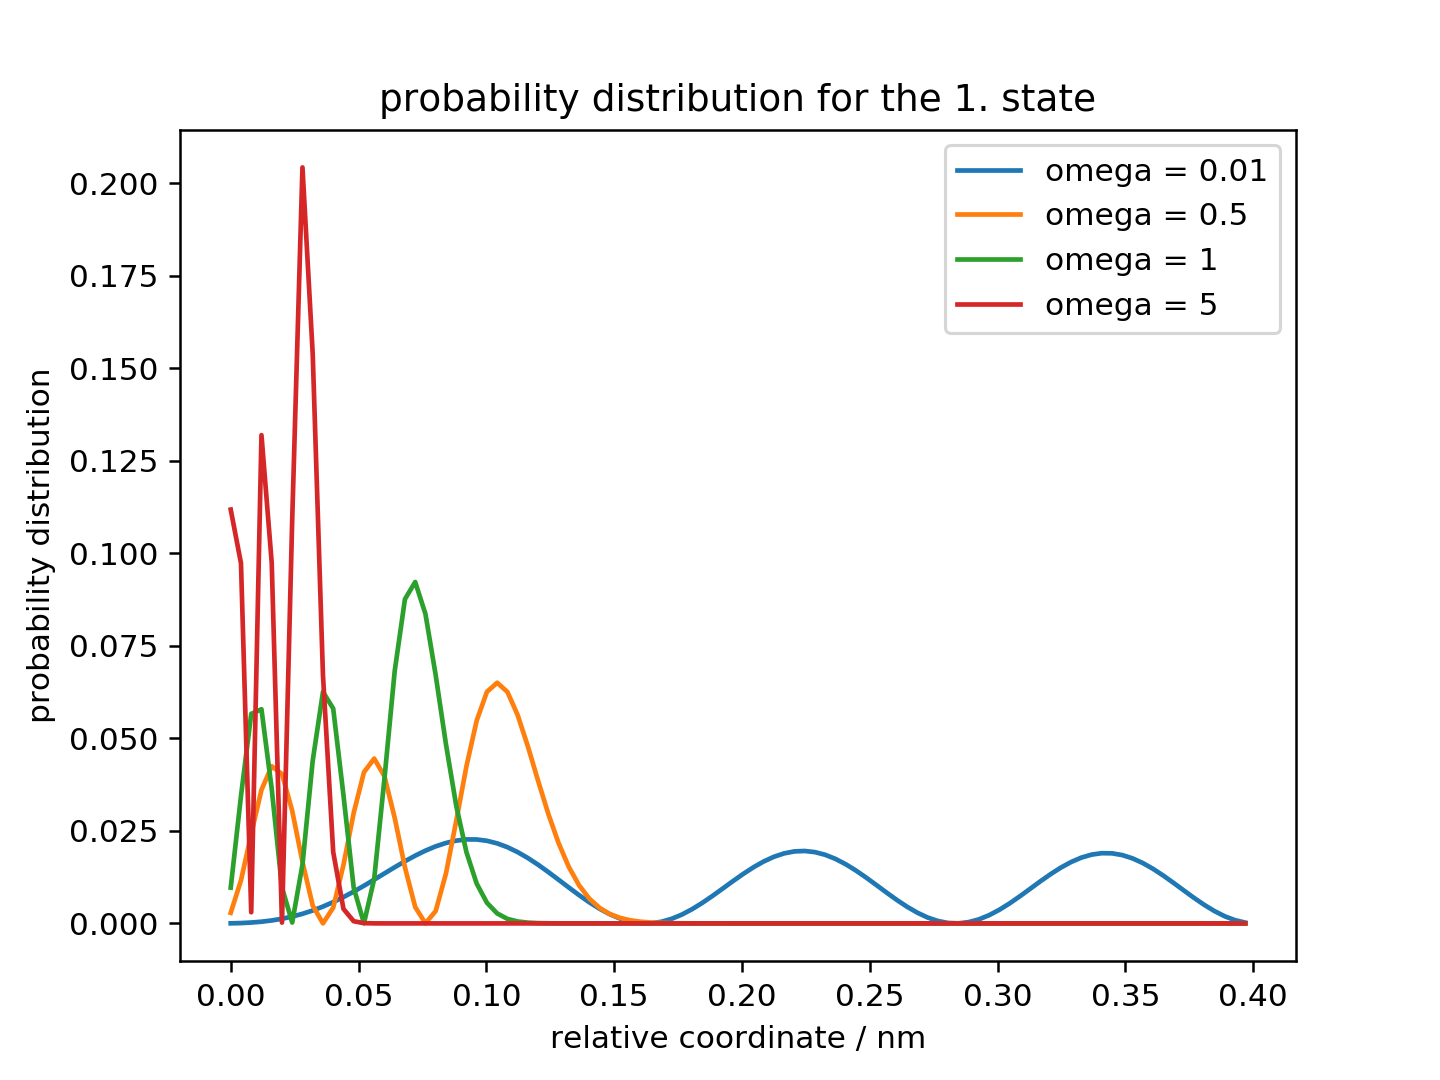
\includegraphics[width=\linewidth]{second_state.png}
  \caption{The probability distribution for two electrons in a potential well, for different potential stengths}
  \label{fig:second_state}
\end{figure}

\section{Conclusion}
The Jacobi method have proven to be useful, but extremely inefficient, for solving my eigenvalue problem. The accurracy of the eigenvalues decrease as the energy state increase, and a solver that not use a full matrix will be better suited to get higher precision for eigenvalues of higher states. I have experienced that in the case of the Schroedinger's equation, $\omega_r$ and $\rho_N$  affect the accurracy of the calculated eigenvalues and eigenvectors. To get a better understnding of how these variables work together, it wold have been easier to work with a faster eigenvalue problem solver. 

\begin{thebibliography}{1}
\bibitem{Projectdescription} 
Hjort-Jensen, M.: Computational Physics: Project 2,
\\\texttt{https://github.com/CompPhysics/ComputationalPhysics/blob/master/doc/Projects/2017/Project2/pdf/Project2.pdf}


\bibitem{Oscillatorfrequancies} 
M. Taut, Phys. Rev. A 48, 3561 (1993),
\\\texttt{https://journals.aps.org/pra/abstract/10.1103/PhysRevA.48.3561}
\end{thebibliography}



\end{document}